\documentclass[12pt]{article}
\usepackage[utf8]{inputenc}
\usepackage{graphicx}
\usepackage{amsmath}
\usepackage{xcolor}
\usepackage{listings}
\usepackage[margin=1in]{geometry}
\usepackage{hyperref}
\usepackage{caption}
\usepackage{subcaption}
\usepackage{titlesec}
\usepackage{booktabs}
\usepackage{float}
\usepackage{afterpage}

\definecolor{codebg}{rgb}{0.95,0.95,0.95}
\definecolor{myblue}{rgb}{0,0.3,0.6}

\lstset{
    backgroundcolor=\color{codebg},
    basicstyle=\ttfamily\small,
    breaklines=true,
    frame=single,
    numbers=left,
    numberstyle=\tiny\color{gray},
    keywordstyle=\color{myblue},
    commentstyle=\color{green!50!black},
    stringstyle=\color{red},
    showstringspaces=false,
    tabsize=4
}

\title{Sunflower Counting Using Color Segmentation and Morphology}
\date{\today}

\begin{document}

\maketitle

\begin{abstract}
This document presents an automated sunflower counting system using color segmentation and morphological image processing. The pipeline includes HSV color filtering, noise removal, and connected component analysis to count sunflowers in an image.
\end{abstract}

\section{Libraries Used}
\begin{itemize}
    \item \texttt{numpy}: For numerical operations and array manipulation
    \item \texttt{cv2} (OpenCV): For image processing and computer vision operations
    \item \texttt{matplotlib.pyplot}: For image visualization and plotting
\end{itemize}

\section{Step-by-Step Process}

\subsection{Step 1: Import Libraries}
\begin{lstlisting}[language=Python]
import numpy as np
import cv2 as cv
import matplotlib.pyplot as plt
\end{lstlisting}

\subsection{Step 2: Download Image}
Download the sunflower field image:
\begin{lstlisting}[language=Python]
!wget https://raw.githubusercontent.com/AsadiAhmad/Sun-Flower-Counter/main/Pictures/sun_flower.jpg -O sun_flower.jpg
\end{lstlisting}

\subsection{Step 3: Load and Display Image}
Load and display the original image:
\begin{lstlisting}[language=Python]
sun_flower = cv.imread("sun_flower.jpg")
plt.imshow(sun_flower[...,::-1])  # Convert BGR to RGB for display
\end{lstlisting}

\begin{figure}[H]
    \centering
    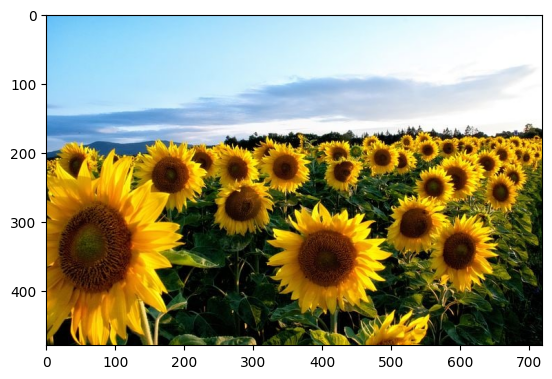
\includegraphics[width=0.8\textwidth]{original_flower.png}
    \caption{Original sunflower field image}
    \label{fig:original}
\end{figure}

\subsection{Step 4: Convert to HSV Color Space}
Transform to HSV for better color segmentation:
\begin{lstlisting}[language=Python]
hsv_sun_flower = cv.cvtColor(sun_flower, cv.COLOR_BGR2HSV)
\end{lstlisting}

\subsection{Step 5: Filter Brown Sunflower Centers}
Isolate brown sunflower centers using HSV range:
\begin{lstlisting}[language=Python]
lower_brown = np.array([0, 50, 0])    # Lower HSV bound
upper_brown = np.array([20, 255, 75]) # Upper HSV bound
masked_sun_flower = cv.inRange(hsv_sun_flower, lower_brown, upper_brown)
filtered_sun_flower = cv.bitwise_and(sun_flower, sun_flower, mask=masked_sun_flower)
\end{lstlisting}

\begin{figure}[H]
    \centering
    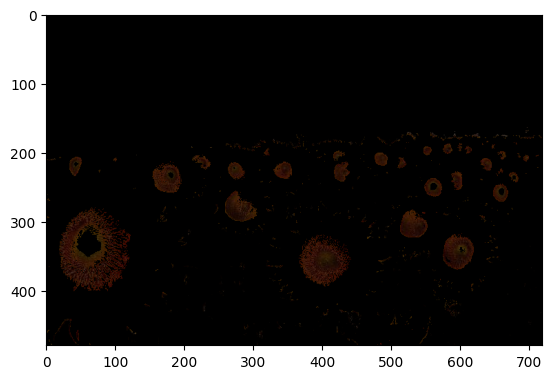
\includegraphics[width=0.8\textwidth]{filtered_flower.png}
    \caption{Image after brown color segmentation}
    \label{fig:filtered}
\end{figure}

\subsection{Step 6-7: Convert to Grayscale and Binarize}
Prepare for morphological processing:
\begin{lstlisting}[language=Python]
filtered_sun_flower_gray = cv.cvtColor(filtered_sun_flower, cv.COLOR_BGR2GRAY)
filtered_sun_flower_bin = np.where(filtered_sun_flower_gray > 10, 255, 0)
scaled_flower_bin = filtered_sun_flower_bin.astype(np.uint8)
\end{lstlisting}

\begin{figure}[H]
    \centering
    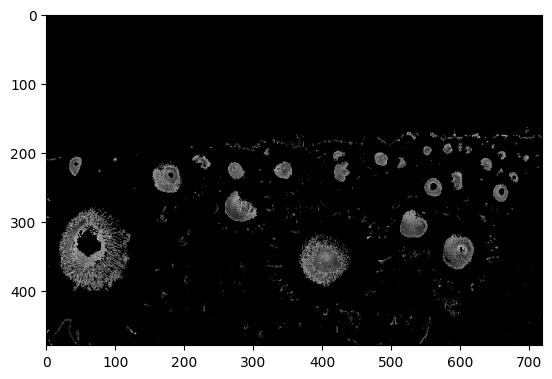
\includegraphics[width=0.8\textwidth]{binary_flower.png}
    \caption{Binarized image of sunflower centers}
    \label{fig:binary}
\end{figure}

\subsection{Step 8-9: Morphological Erosion}
Remove small noise artifacts:
\begin{lstlisting}[language=Python]
erosion_kernel = np.ones((2, 2), np.uint8)
erosion_sun_flower = cv.erode(scaled_flower_bin, erosion_kernel, iterations=3)
\end{lstlisting}

\begin{figure}[H]
    \centering
    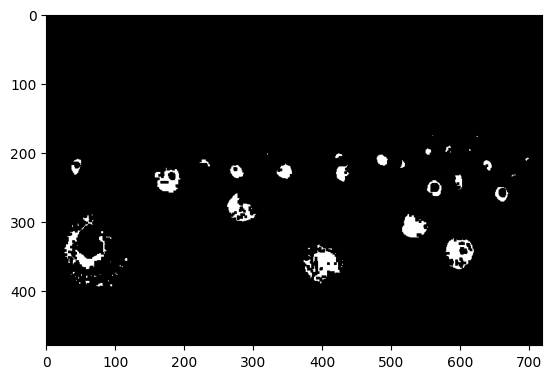
\includegraphics[width=0.8\textwidth]{eroded_flower.png}
    \caption{Image after erosion (noise removal)}
    \label{fig:eroded}
\end{figure}

\subsection{Step 10: Morphological Dilation}
Connect broken parts of sunflower centers:
\begin{lstlisting}[language=Python]
dilation_kernel = np.ones((3, 3), np.uint8)
dilation_sun_flower = cv.dilate(erosion_sun_flower, dilation_kernel, iterations=5)
\end{lstlisting}

\begin{figure}[H]
    \centering
    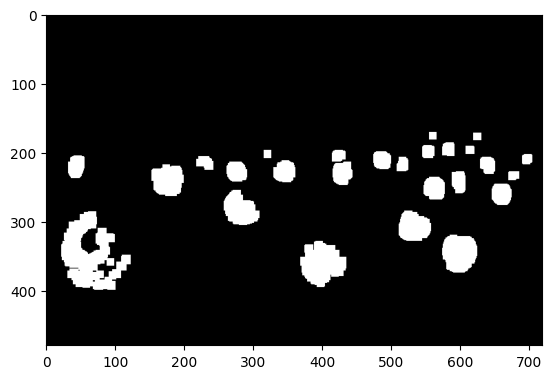
\includegraphics[width=0.8\textwidth]{dilated_flower.png}
    \caption{Image after dilation (connecting parts)}
    \label{fig:dilated}
\end{figure}

\subsection{Step 11: Counting Sunflowers}
Count connected components:
\begin{lstlisting}[language=Python]
num_labels, labels = cv.connectedComponents(dilation_sun_flower)
flower_count = num_labels - 1  # Subtract background
print(flower_count)
\end{lstlisting}

Output:
\begin{verbatim}
26
\end{verbatim}

\subsection{Step 12: Calculating Accuracy}
Calculate counting accuracy:
\begin{lstlisting}[language=Python]
percent = (flower_count/29)*100
print(f'{percent:.2f}%')
\end{lstlisting}

Output:
\begin{verbatim}
89.66%
\end{verbatim}

\section{Technical Explanations}

\subsection{Image Processing Pipeline}
\begin{itemize}
    \item \textbf{HSV Color Space}: Better for color segmentation than RGB
    \item \textbf{Brown Color Range}: Carefully tuned to capture sunflower centers
    \item \textbf{Morphological Operations}: Erosion removes noise, dilation connects parts
    \item \textbf{Connected Components}: Counts individual sunflower centers
\end{itemize}

\subsection{Performance Notes}
\begin{itemize}
    \item 89.66\% accuracy achieved on sample image
    \item Color range selection critical for good segmentation
    \item Kernel sizes and iterations affect counting results
\end{itemize}

\begin{center}
    \href{https://github.com/AsadiAhmad/Sun-Flower-Counter}{
        \includegraphics[width=0.2\textwidth]{github_logo.png} \\
        \texttt{https://github.com/AsadiAhmad/Sun-Flower-Counter}
    }
\end{center}

\end{document}